% ------------------------------------------------------------------------------
% Chapter 1
% Delete this content and replace with your own
%tis is a test sentence
% ------------------------------------------------------------------------------
\chapter{Introduction} % enter the name of the chapter here
\label{cha:introl} % enter the chapter label here (for cross referencing)

% \input{background}

\begin{figure}
    \centering
    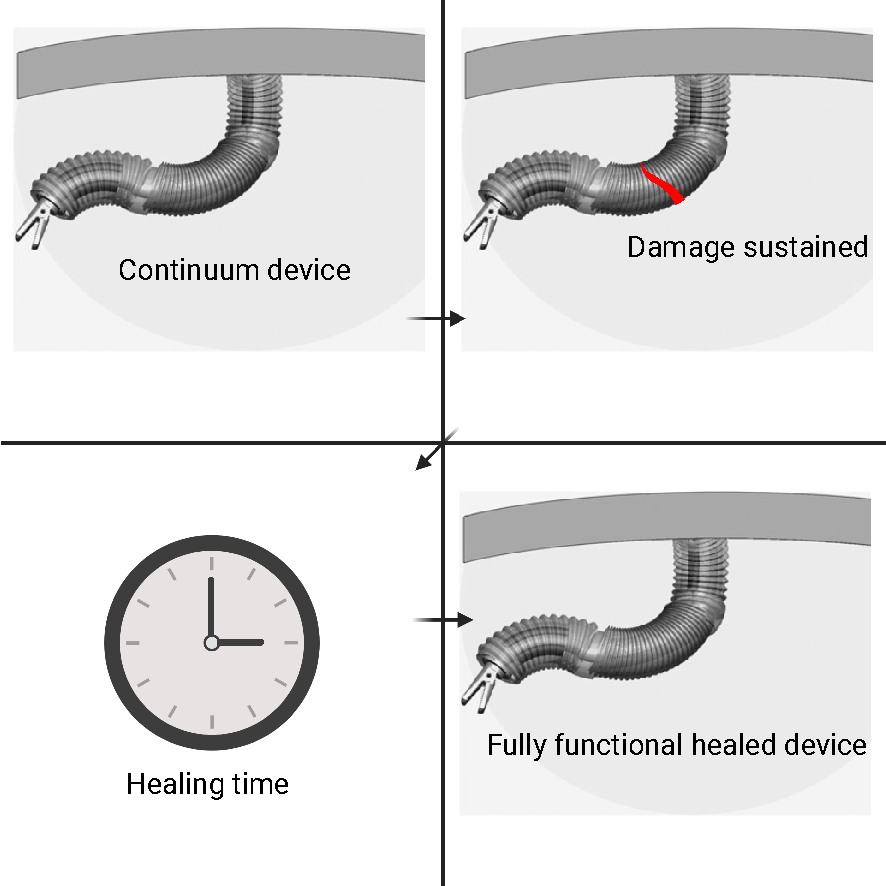
\includegraphics[width=0.8\linewidth]{Images/overview v3.pdf}
    \caption{A continuum device sustaining damage before self-healing and regaining full functionality using a modified image from \cite{cianchetti2014soft}}
    \label{fig:overview}
\end{figure}

\section{Importance and Applications of Soft Robotics}
Soft robots are devices known for their use of soft materials, compliant nature and near infinite degrees of freedom. Degrees of freedom (DOF) is a term related to the number of independent movements a robot can make in 3D space \cite{lynch2017modern}. Soft robots are usually nature inspired such as ``vine-like'' tip growing robots \cite{hawkes2017soft, davy2025magnetic}, ``snake like'' continuum robots \cite{anderson1967tenser, lloyd2020learnt} and ``hand-like'' soft grippers \cite{ilievski2011soft, guo2018soft}. The advantages of using a body that is highly deformable and with near-infinite DOF means these devices can be actively controlled to navigate tortuous environments with ease. 

This report focuses on continuum robots, often characterised by their long flexible bodies, commonly used for navigation and delivery or retrieval of objects in constrained environments \cite{russo2023continuum}. Continuum robots can be classified into ``continuous backbone'' and ``segmented back-bone'' designs \cite{russo2023continuum}. Continuous backbone devices are made from a soft and compliant material, in this report we will call these ``soft-bodied'', whereas, a segmented backbone refers to those that are made from hard, inflexible segments that are flexibly attached to achieve high curvatures, referred to here as ``hard-bodied''.

Hard-bodied continuum robots benefit from stiffer materials allowing a greater ease of control \cite{russo2023continuum} which can improve dexterity. However, they do not easily deform and are therefore more likely to impart a greater force on the surrounding environment \cite{davy2024vine}.  Hard continuum robots are often tendon driven, whereby the segments are joined by wires that can be pulled to give specific movements. Whereas soft bodied continuum robots can achieve high curvatures and low forces on surroundings \cite{rus2015design}, but are often harder to control due to their methods of actuation \cite{russo2023continuum} and can suffer from material failure \cite{abidi2017intrinsic}. Soft continuum robots commonly take the form of an inflated body, these can be controlled in many ways such as varying pressure \cite{hawkes2017soft}, strain limiting a specific region \cite{guo2024encoded, dean2025anisotropic} or magnetic actuation \cite{davy2025magnetic, davy2024vine}. Pressurised systems that rely on fluids need a constant seal to maintain function as opposed to a segmented tendon driven approach that can be partially damaged and remain actuatable. This motivates the utilisation of resilient materials, such as self-healing polymers, for soft robotic contexts.



\section{Types of Self-Healing Polymers}

\begin{figure}
    \centering
    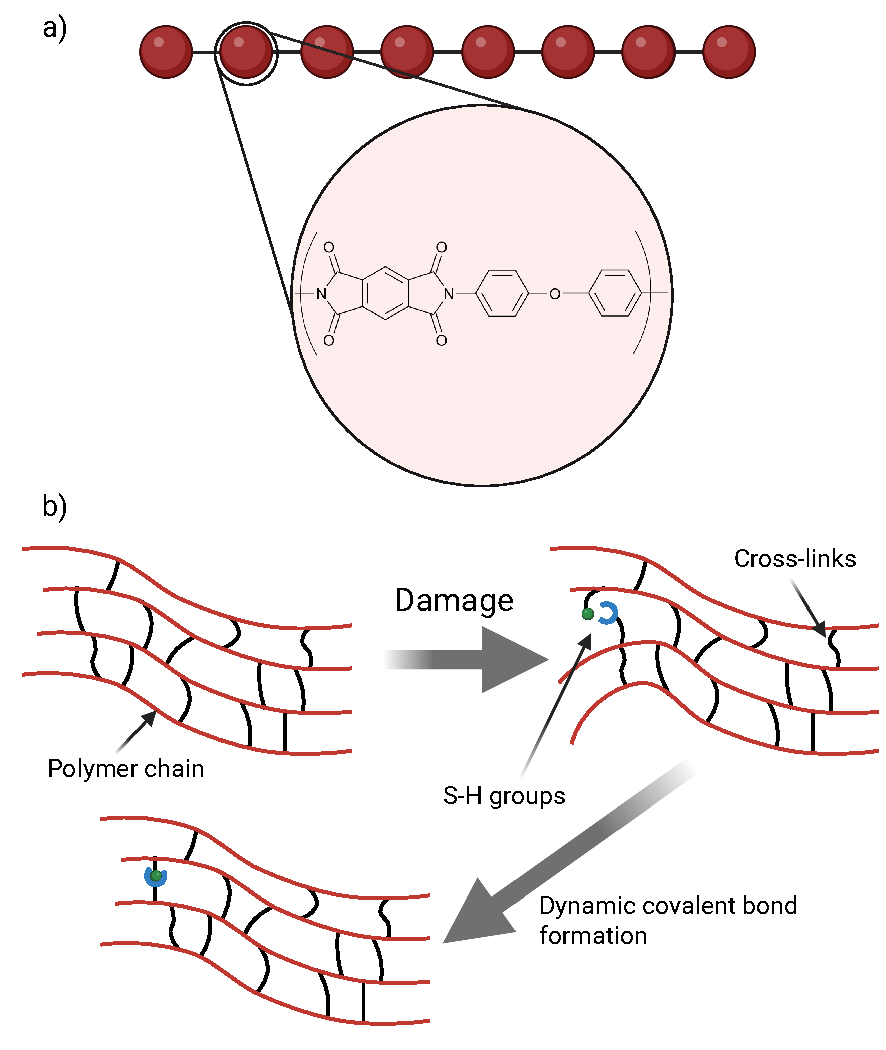
\includegraphics[width=1\linewidth]{Images/Self healing polymer.pdf}
    \caption{a) The polymer chain with a repeating chemical sub-unit. b) The mechanism of damage and repair for a self-healing polymer}
    \label{fig:shpolymer}
\end{figure}

Polymers are a type of molecule that consists of several repeating sub-units, these form chains that are combined many times over to form materials. Self-healing (S-H) polymers are a type of polymer that can heal damage \cite{srivastav2025comprehensive}. This occurs through reactions and interactions between multiple polymer chains to reconnect chains that have been shifted apart through damage. The process of damaging or cutting a polymer does not break bonds in the polymer backbone but instead can break interchain interactions called cross-linking, allowing the chains to drift apart, reforming the cross-linking interactions will ``heal" the material \cite{binder2013self}. 

S-H polymers can be classified into intrinsic or extrinsic healing, and autonomous or non-autonomous \cite{terryn2021review}. Materials with an intrinsic healing capacity involve a healing mechanism through chemical bonds or interactions that are continuously present in the polymer, rather than extrinsic healing, such as capsules of ``healing" material that are broken through damage and causing the material to reform \cite{white2001autonomic}. Autonomy refers to the healing process occurring without external input. For example, capsules that burst upon damage of the material and release a healing agent are classified as autonomous, whereas a photochemical reaction that needs UV light to activate \cite{trenor2004coumarins,froimowicz2011photoreactive} is a non-autonomous mechanism. 


\section{Comparison of Different Self-Healing Pathways}
There are a variety of different pathways that can be taken to create a S-H polymer depending on the chemistry of the initial polymer. The pathways that will be focused on are intrinsically self-healed types, however, both autonomous and non-autonomous types will be considered.

The three pathways below rely on a property of some electrons called conjugation. Conjugation occurs when specific electron orbitals overlap in such as way that allows the electrons to move around the molecule. This is often exploited with a property of some atoms called electronegativity, having a highly electronegative atom in a molecule will attract conjugated electrons to create a local high density region of electrons and therefore a polarisation in a molecule. 

Dynamic covalent bonds can form and break based on the conditions applied to them \cite{guo2025diels} and they are ideal for use as mechanisms for S-H due to their intrinsic nature and reliability in production of high yields \cite{nicolaou2002diels}. This report investigates the use of two types of dynamic covalent bonding, Diels-Alder and Michael additions, and an example of a supramolecular interaction. Supramolecular chemistry is based on interactions that are non-covalent and may be more suited to a soft material \cite{yang2018self}. This is due to the self-healing mechanism of the cross-links that forms interactions therefore the polymer chains can move semi-independently \cite{wanasinghe2022dynamic,yang2018self}. Whereas, a dynamic covalent bond has a much higher bond energy \cite{guo2025diels} and can therefore get closer to the original physical properties of a polymer.

\subsection{Using a Diels-Alder Addition as a Self-Healing Pathway}

\begin{figure}
    \centering
    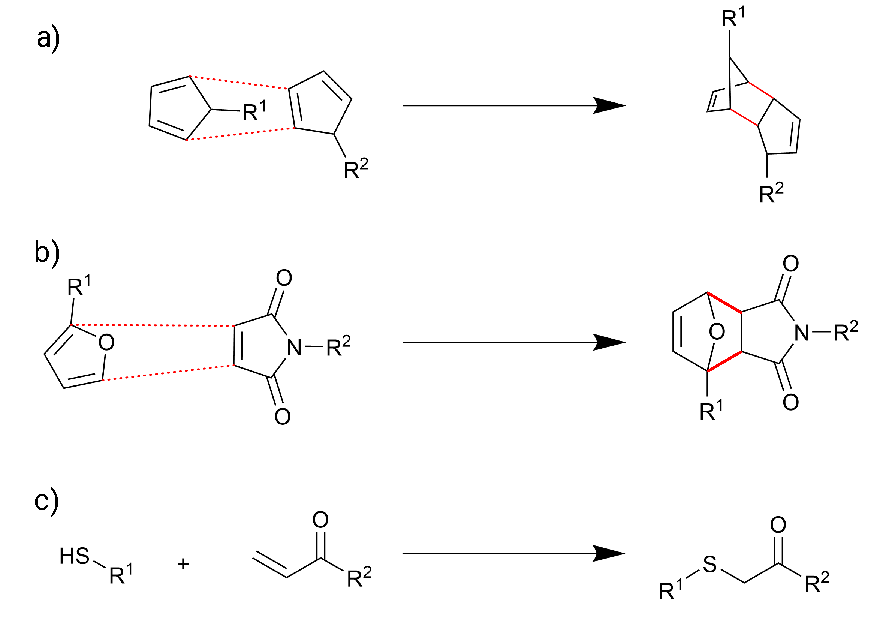
\includegraphics[width=0.8\linewidth]{Images/DA reactions.pdf}
    \caption{a) A Diels-Alder reaction between two molecules of cylopentadiene. b) A Diels-Alder reaction between a furan and maleimide. c) A Thiol-Michael Addition between a thiol and a conjugated alkene. }
    \label{fig:dareactions}
\end{figure}
Diels-Alder (DA) reactions require a diene, a class of molecule characterised by having two sets of double bonds, and an alkene (``dieneophile") \cite{ratwani2023self,guo2025diels}. The reaction occurs when conjugated electrons from the diene are free to move to form new bonds with the carbons either side of the alkene double bond, this creates a new ring structure. A faster reaction is generally observed with an electron rich diene and an electron poor dienophile \cite{briou2021trends}. The electronic character of the reagents can be altered by changing their local substituents. This class of reactions can have lots of different conditions depending on the molecules involved. Some variations can occur at room temperature \cite{huertas2009solvent}, which may make them an ideal choice for an autonomously healed medical device as the healing can occur whilst deployed in the body. However, many DA reactions are light \cite{trenor2004coumarins,froimowicz2011photoreactive} or heat activated \cite{li2014situ}.

Some molecules such as cyclopentadiene can perform a DA reaction with itself, this has the potential to be an ideal choice for a S-H polymer as the molecule will never be in close proximity to a molecule that it cannot react with. However, some evidence has shown that the bonds formed are not very strong and therefore high tensile strength materials may not be possible \cite{ratwani2023self}.

One of the most common types of DA reaction is a heat activated reaction between a derivative of both furan and maleimide \cite{ingoglia2014microencapsulation}. They react extremely accurately and require mild conditions \cite{ratwani2023self}, therefore they are very suitable for application as a robotics material.
One of the reasons that this reaction is so effective is that the maleimide has electron withdrawing carbonyl groups which make the dieneophile electron poor and therefore reacting faster. However, this mechanism has a disadvantage compared to cyclopentadiene as there are two halves of the end product. Therefore, there must be two different processes occurring to create both the furan substituted and maleimide substituted chains. This increases the number of total steps in the reaction which increases the risk of low reaction yields and wasted material. 


\subsection{Using a Thiol-Michael Addition as a Self-Healing Pathway}
Thiol Michael additions are a type of reaction that relies on a thiol, a molecule characterised by a sulfur containing group and a conjugated alkene \cite{nair2014thiol}. The conjugated alkene used in a Michael addition is with a carbonyl group that will attract the electrons from the alkene to allow the thiol group to react. This has a similar advantage to the Diels-Alder reaction that it is not totally dependant on specific reactants merely groups of reactants. Therefore slight changes can be made to the adjoining groups to tweak the reaction conditions. This has been previously shown to have been successful with a heat activated reaction that could heal scratches after 15 to 30 minutes at 60 \degree C \cite{kuhl2016self}. 

\subsection{Using a Pi-Stacking Approach as a Self-Healing Pathway}
Pi-Stacking is a type of intermolecular interaction whereby conjugated systems interact based on the neighbouring substituents determining if a region is electron rich or poor. These electron disparities cause an electrostatic interaction. This method commonly uses pyrenyl groups, these are polycyclic aromatic compounds, a very pi-electron rich species. These can be interacted with a napthalene diimide complex, an electron poor pi-system to give four pi-stacking interactions. A method has shown the creation of a polymer chain end group which can sandwich a napthalene group within two pyrenyl groups. \cite{burattini2011supramolecular}. This method can be combined with other intermolecular interactions like hydrogen bonding \cite{yuan2025self} or mettalosupramolecular interactions to give a stronger interaction \cite{mei2016highly}.


\section{Applications of Self-Healing Polymers in Soft Robotics}

Continuing the theme of biological inspiration of soft robotics, S-H polymers can be used to extend the lifespan of components. In soft continuum robots, the goal is usually to make the robot softer than the environment surrounding it \cite{rus2015design}. This presents challenges in abrasive environments that can damage the device. It is therefore evident that a damage resilient material would be useful. Damage resilient materials can take multiple forms: Damage isolation, material elasticity, physical self healing such as low melting temperature materials and chemical self healing \cite{bilodeau2017self}.



\subsection{State of the Art Self-Healing Soft Robots}
 State-of-the-art approaches using intrinsic S-H mechanisms are commonly based on DA chemistry \cite{terryn2021review}. These have been successfully implemented in tendon-driven \cite{roels2019multi} and pneumatically controlled soft robotic devices \cite{terryn2020room, terryn2017pneumatic}. Such devices are capable of recovering from macroscopic damage, including punctures and cuts. Additionally, there are non-covalent approaches that utilize hydrogen bonding in the development of soft self-healing actuators, such as in McKibben muscle designs \cite{lopez2020autonomous}.

\subsection{Requirements for Self-Healing Polymers in Soft Robotics}
Terryn \textit{et al.} \cite{terryn2021review} states that there are 5 main criteria for a S-H polymer; macroscopic damage must be healed completely; healing can take place multiple times at the same location; there are minimal material property changes after healing; elastomeric behaviour is achieved; the reprocessing and recycling of a material is possible. Here we propose that elastomeric behaviours are non-essential and a more useful requirement would involve a timely S-H reaction.  


\section{Limitations with Current Materials for Soft Robotics}

Damage control whilst a device is active can be a challenge \cite{kashef2025toward}, this shows a need for autonomous S-H \cite{terryn2021review}. Non-autonomous S-H can be made ``functionally autonomous" through the use of stimuli responsive mechanisms, however, the current options are slow in operation \cite{kashef2025toward}. Currently recovery timescales of applied S-H polymers are around 25 hours \cite{terryn2017pneumatic, bilodeau2017self}. By altering the polymer used or S-H pathway this could be improved. There is also a lack of an easy synthesis route for many of the current polymer options \cite{bilodeau2017self}, thereby increasing the cost and reducing widespread use. Also the number of damage-repair cycles in these devices are low, such as 3 or less \cite{terryn2017pneumatic}. Most devices do not achieve all five criteria laid out in the Terryn \textit{et al.} review \cite{terryn2021review}, such as the McKibben design of A. Lopez Diaz \textit{et al.} \cite{lopez2020autonomous} only reporting a healing efficiency of 65\%.
